% Ημερίδα πρακτικής άσκησης με δεδομένα από το CERN - Σάββατο 7 Μάρτη 9:00 - 17:00
\begin{MyArticle}[enhanced, tikz={rotate=0}, width=0.3\textwidth]{Master of Masterclasses}
  \begin{multicols}{2}
    Another particle physics masterclass was organized at the University of Cyprus
    by Professor Fotios Ptochos for the 8$^{th}$ year
    in a row. It took within the framework of the IPPOG effort,  with
    the aim of informing young students about the research being
    carried out at CERN and the wider field of Particle Physics.
    Department of Physics. The event you took place on Saturday 07 March
    2020 at the University of Cyprus Campus between 9:00 - 17:00. It 
    included lectures about the world of elementary particles,
    detection methods, and the technology developed starting with
    basic research in both this and related fields of physics. Students had a unique opportunity to
    analyze data from proton-proton collisions, as recorded by the CMS
    detector at CERN's LHC. They discussed their
    findings with students from other countries as well as scientists
    at CERN through a video conference.
    % ========================
    \begin{figure}
      \begin{center}
        \leavevmode
        %\includegraphics[width=0.45\textwidth]{./figures/Fotis6.png}
        %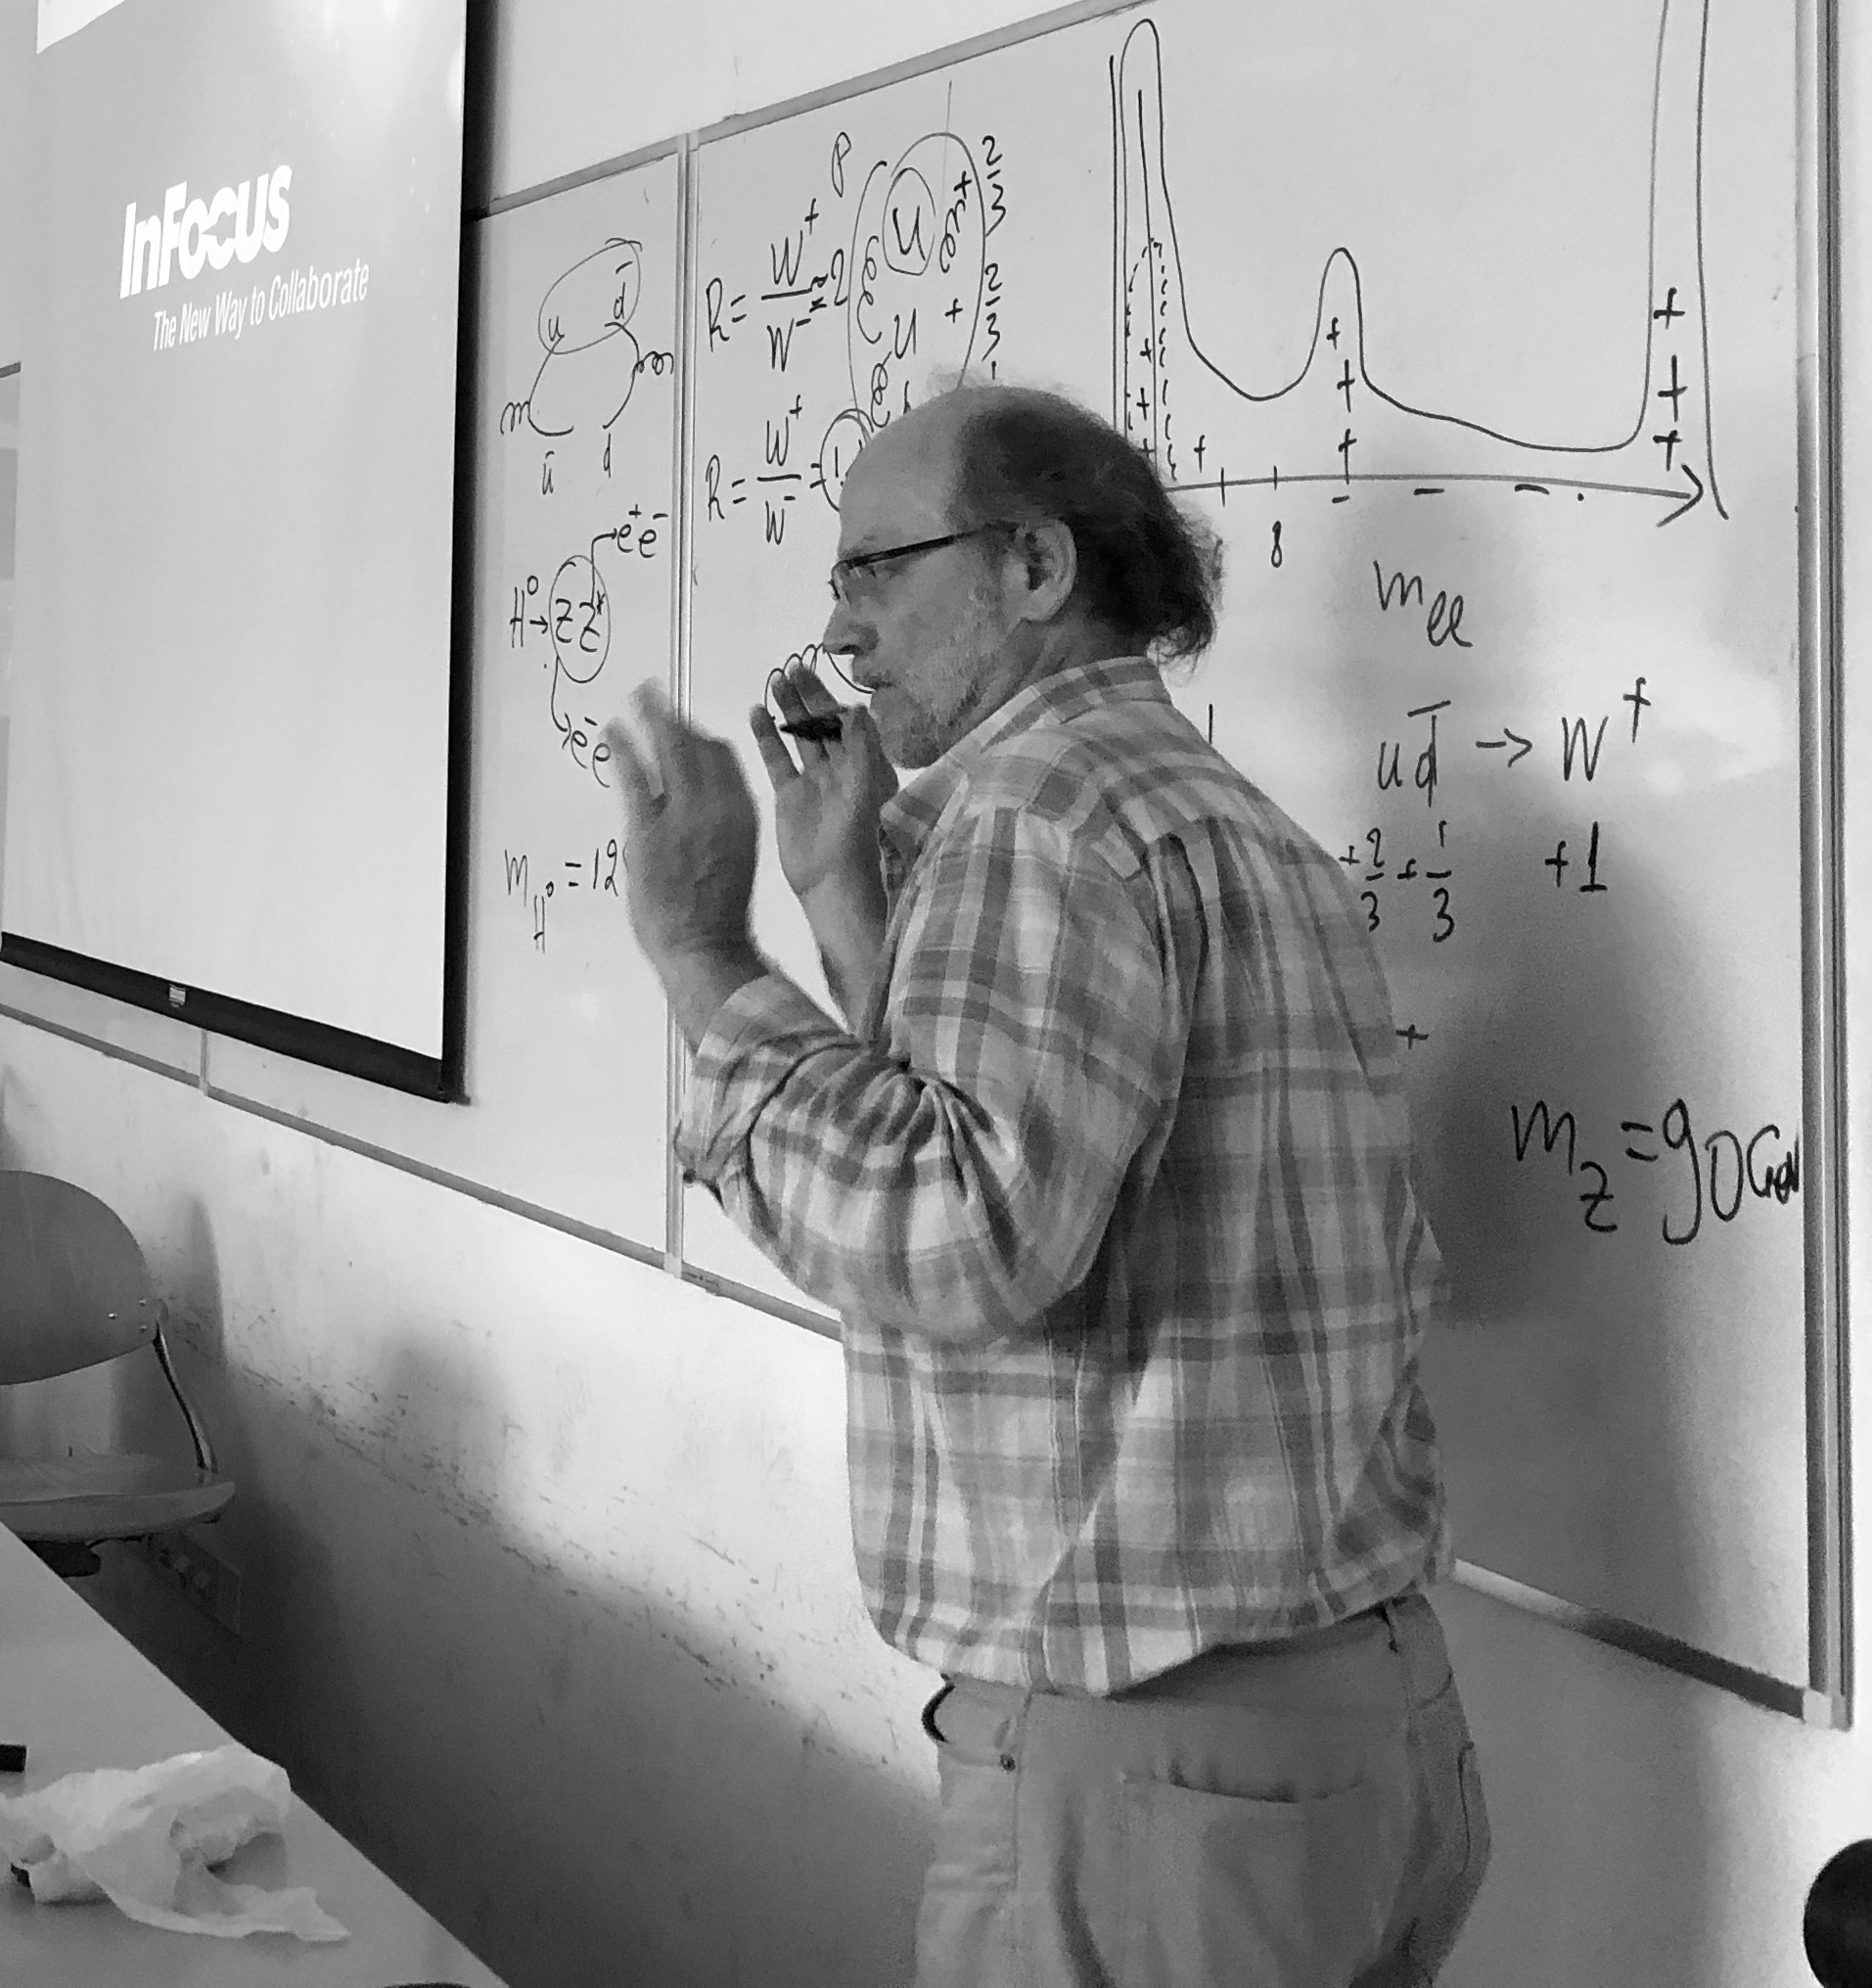
\includegraphics[width=0.5\textwidth]{./figures/Fotis6-narrow.png}
        %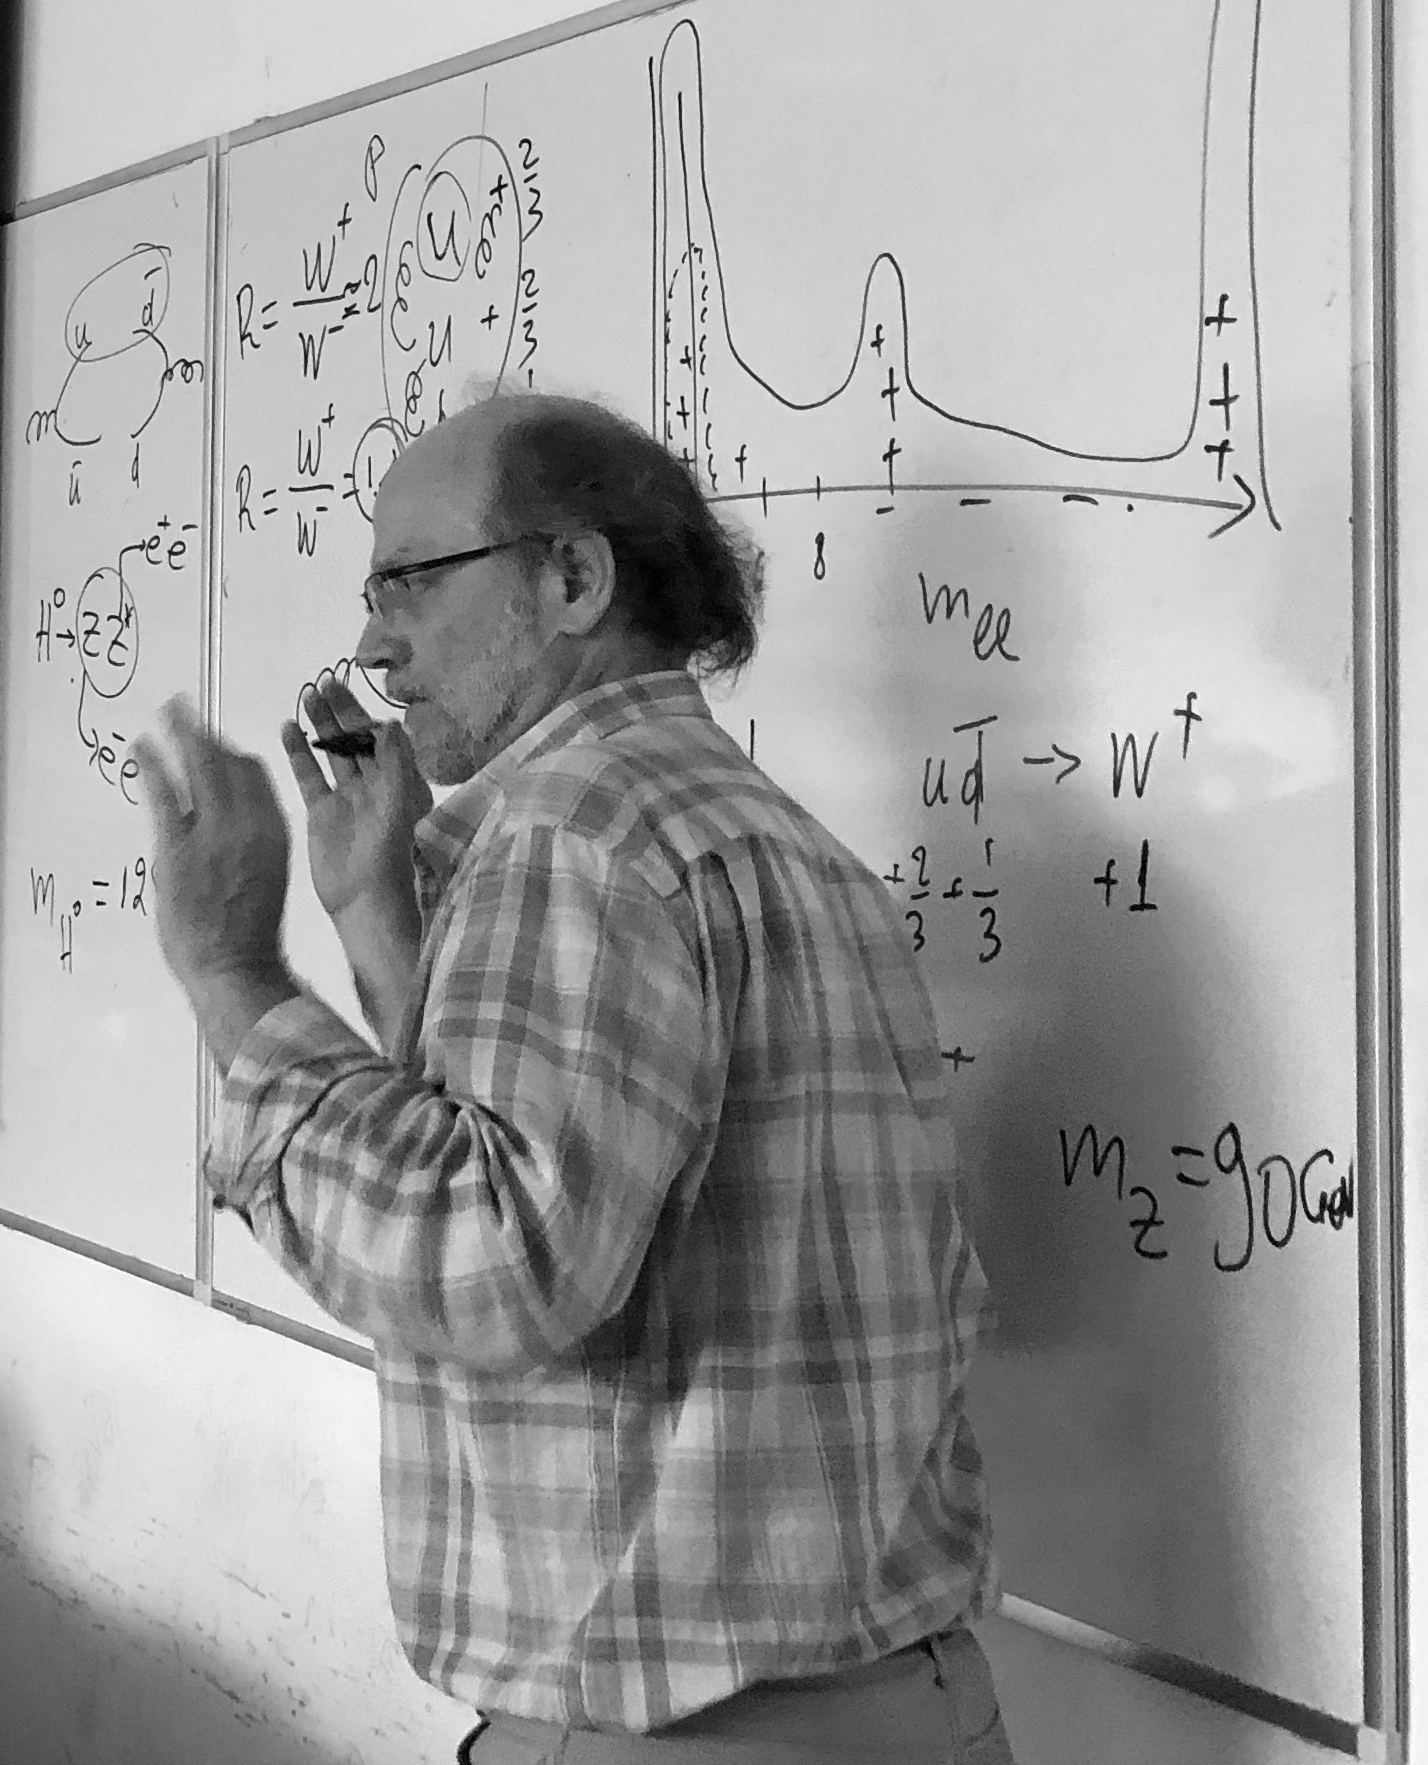
\includegraphics[width=0.4\textwidth]{./figures/Fotis6-small.png}
        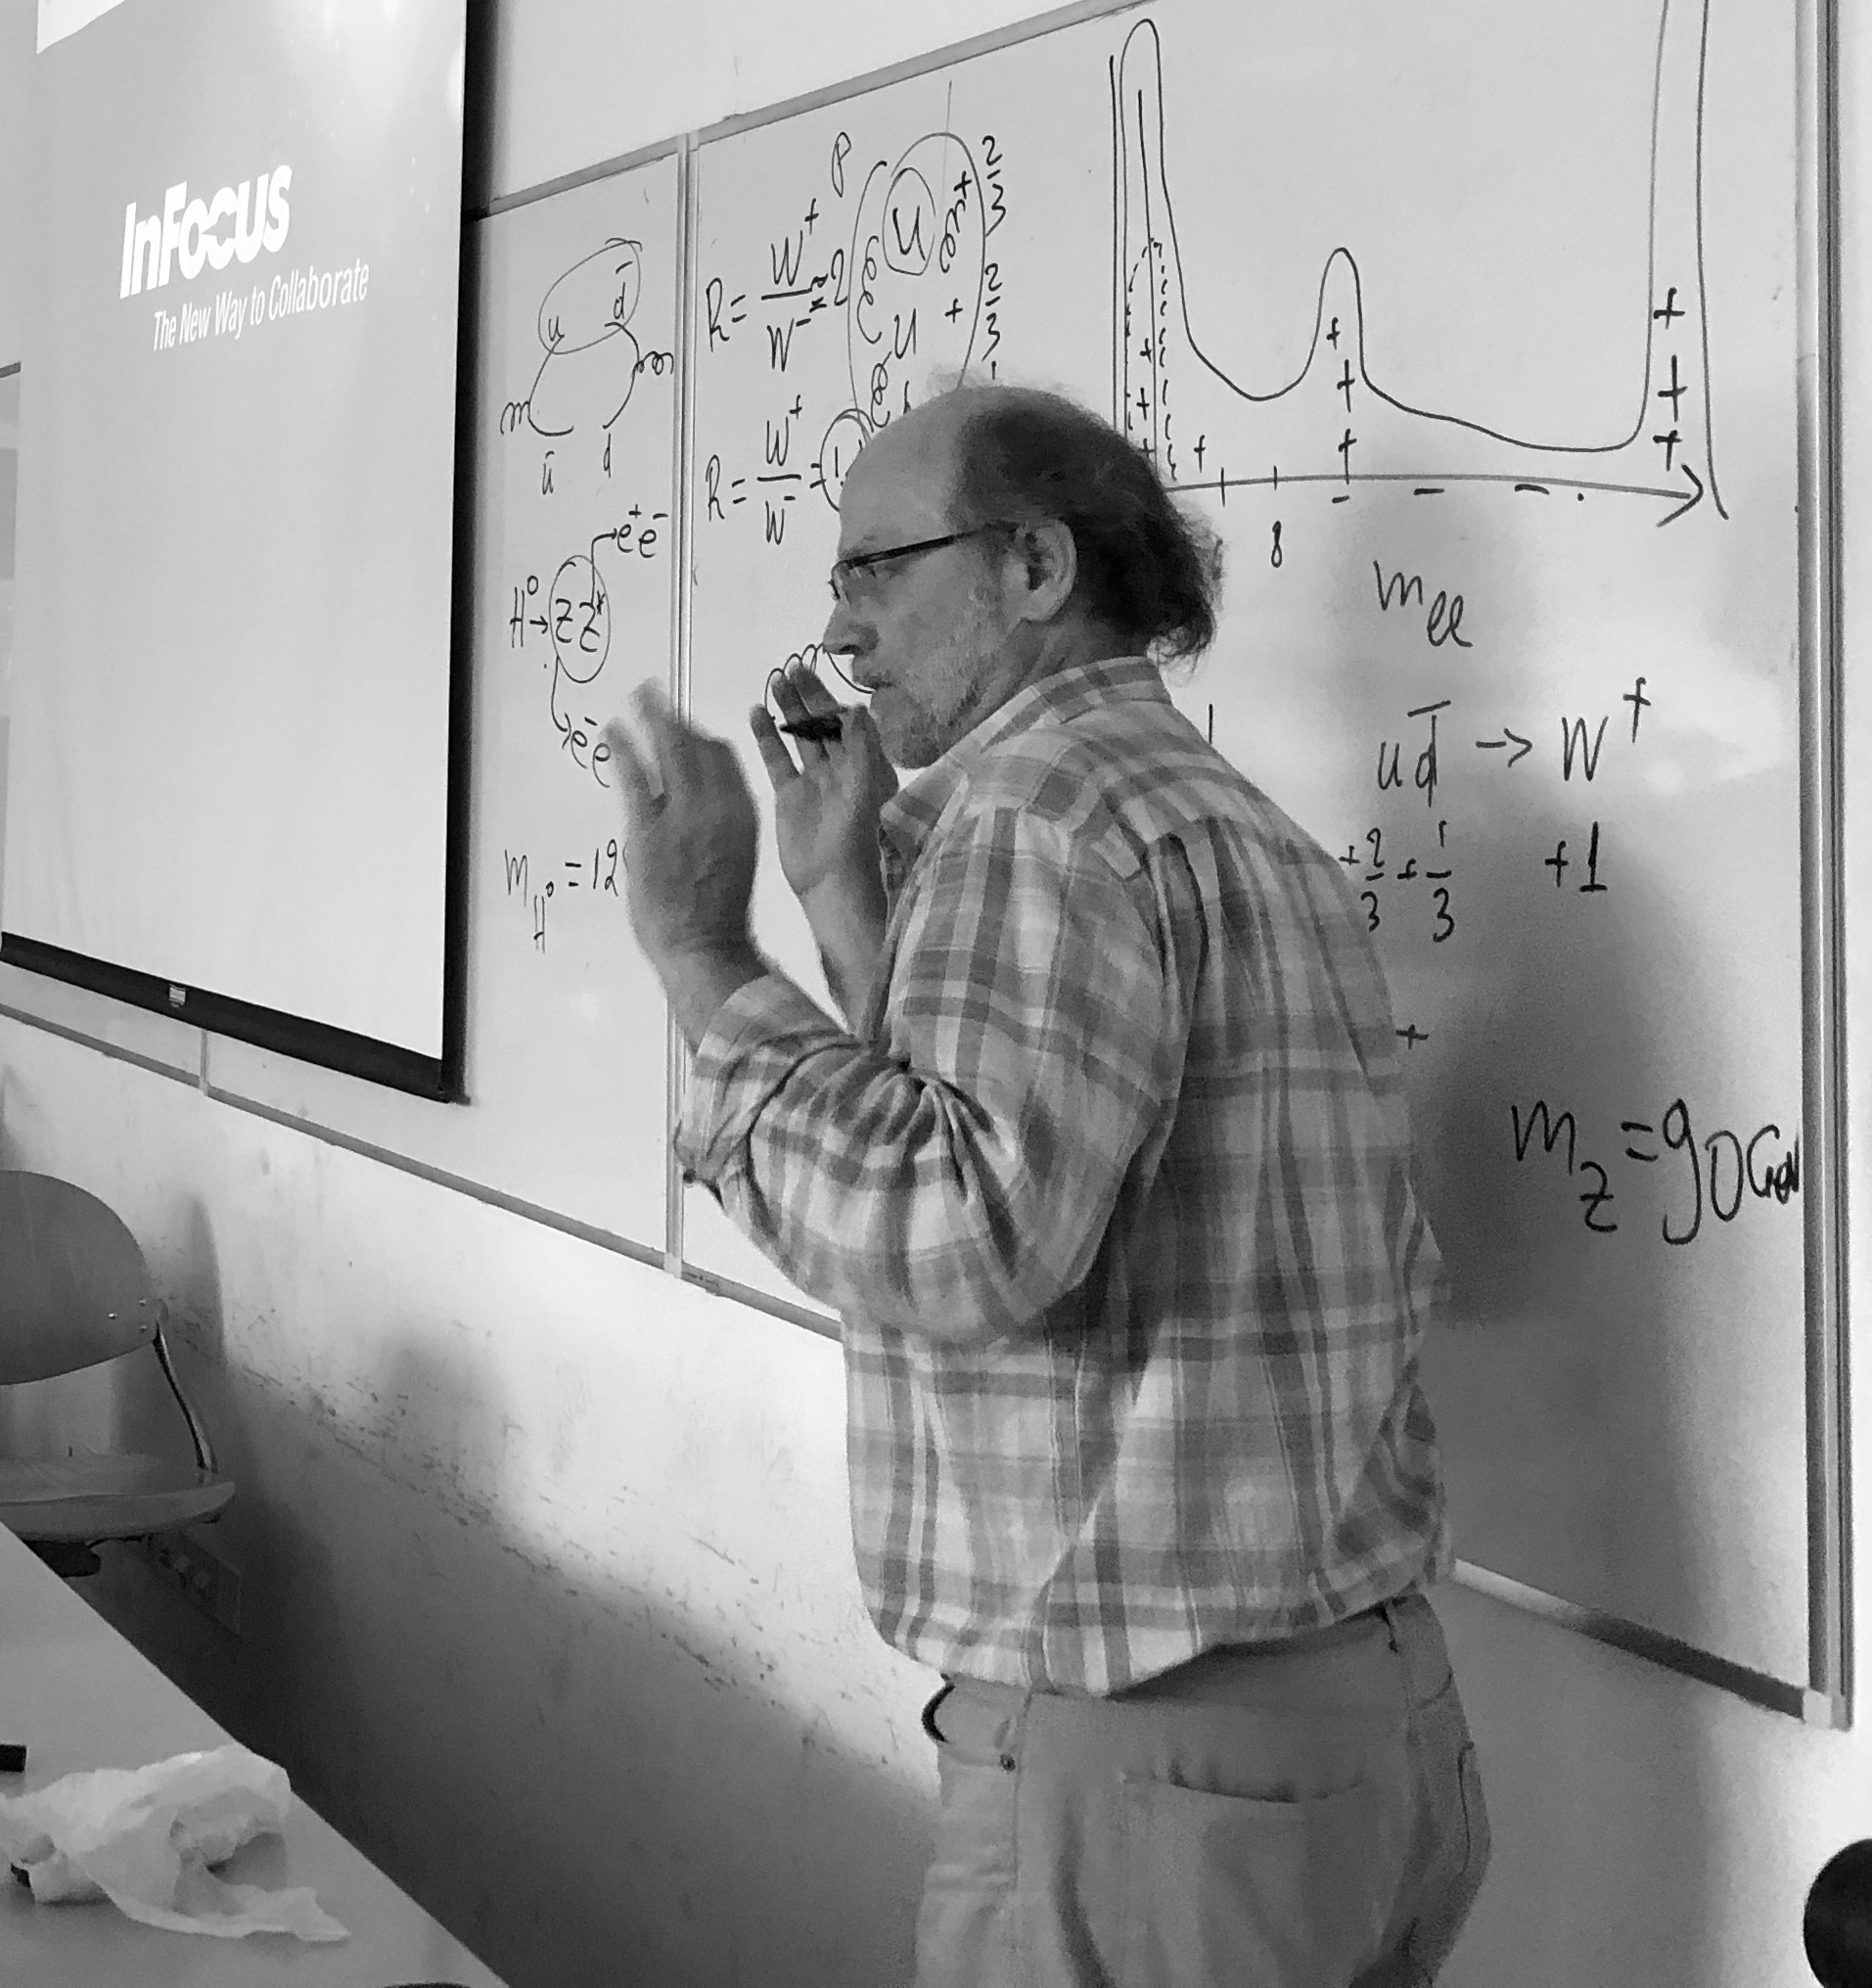
\includegraphics[width=0.4\textwidth]{./figures/Fotis6-narrow.png}
      \end{center}
    \end{figure}
    % ========================
  \end{multicols}
\end{MyArticle}
